%\appendix 
%only needed once to demarcate start of appendix chapters

\chapter[Reconstructing Ancestral Histories]{Reconstructing Ancestral Histories Under Multivariate Brownian Motion}

\label{app:App3}

\clearpage

\section{Motivation}

When simulating under a multivariate Brownian motion model of character evolution, the location of the resultant continuous character alignment is marginalized out during phylogenetic likelihood calculation with the Felsenstein Pruning Algorithm, because if both the root state and location are unknown, the full likelihood is completely non-identifiable with respect to either. Adding the same value to all tip characters changes the likelihood not at all, so it matters not what arbitrary value is assigned to the root of the tree. When those continuous characters are passed through an ordinalization filter, however, there arises a strong dependency between the location of the root state and the phylogenetic likelihood, and with it our ability to estimate focal model parameters. This is because the locations of the latent liabilities relative to the locations of the thresholds determine which discrete characters are expressed. Shifting the root state can dramatically change which discrete traits are expressed without a concordant shift in the locations of the thresholds, and so if we wished to simulate fictitious data in an empirically realistic manner, we might wish to fix the thresholds to their estimated values, leaving open the question of where and with what value to set the root.

The location of the root is still non-identifiable, so, as mentioned in the main text, we arbitrarily performed midpoint rooting. The most convenient values to fix its state to for the purpose of estimating between trait correlations, threshold locations, and tip means would be intermediate between the minimum and maximum thresholds, but empirical realism does not beget convenience. Instead, the most principled root state would be that implied by the root's location, midway between the most distantly separated tips, conditional on the observed values throughout the rest of the tree and the character evolutionary process. The multivariate Brownian bridge passing through the root, then, on its way between the tips.

\clearpage

\section{Algorithm}

Finding the parameters of this distribution is straightforward --- one needs only to recall that under multivariate Brownian motion, the tips are drawn from a multivariate normal random variable whose mean is the root state and whose covariance matrix is the Kronecker product of the phylogenetic covariance matrix and the Brownian motion rate matrix. Because of the pulley principle, one can arbitrarily reroot the tree at any tip and equivalently say that the remaining tip data, along with the unobserved state at the midpoint root, are multivariate normal distributed with mean at the observed tip and covariance matrix the Kronecker product of the \textit{new}, rerooted tree and the Brownian motion rate matrix. Depending on the order one took the Kronecker product, as well as the order of the columns in the phylogenetic covariance matrix, one needs to then permute our multivariate normal distribution's covariance matrix into block form, such that those indices corresponding to unobserved characters at the root are found in the upper left corner. Then, one case use known formulae for conditional distributions of multivariate normals to compute the conditional mean and covariance at the root, where if one has a multivariate normal distribution with mean $\mu$ and covariance matrix $\Sigma$, partitioned as

{\large\[\mu_{all} = \begin{bmatrix}
\mu_{1} \\
\mu_{2} \\
\end{bmatrix} \
\Sigma = \begin{bmatrix}
\Sigma_{11} & \Sigma_{12}\\
\Sigma_{21} & \Sigma_{22}\\
\end{bmatrix}
\]}

and realizations partitioned as

{\large\[x = \begin{bmatrix}
x_{unobs} \\
x_{obs} \\
\end{bmatrix}\]}

The distribution of $x_{unobs}$ given $x_{obs}$ is itself multivariate normal, with means and covariance matrix:

{\large\[\mu_1' = \mu_1 + \Sigma_{12}\Sigma_{22}^{-1}(x_{obs}-\mu_2)\]}

{\large\[\Sigma_{11}' = \Sigma_{11} - \Sigma_{12}\Sigma_{22}^{-1}\Sigma_{21}\]}

This is the same relation exploited by the Felsenstein Pruning Algorithm to diagonalize the phylogenetic covariance matrix, only it computes conditional distributions conditional upon values at descendant nodes, rather than on tips also descended from sister branches. 

\clearpage

\section{Additional Applications}

One character history of particular interest to paleontologists and neontologists alike might be the truncated biogeographic diffusion history separating taxa distributed across some geographic range, especially under hypotheses of correlation between geographic (e.g. latitudinal) and morphological variables. Fitting a Brownian motion model to such data can help to investigate latitudinal trends in body shape and size in a phylogenetically sensible way, elegantly avoiding pseudoreplication problems encountered when failing to take phylogeny or population history into account. But naively specifying a multivariate Brownian motion over the whole of $R^n$ does not respect geographic boundaries that might impede an organism's travel, such as mountains, deserts, and oceans (Figure \ref{fig:truncBrownMot}). Preliminary work found that it was possible and efficient to perform data augmentation over internal geographic and morphological states with sufficient granularity as to avoid ocean-faring and mountain-hopping voyages by rejection sampling biogeographic diffusion histories that were consistent with these boundaries. As most such histories would be invalid at high granularity, one could instead rejection sample single locations at a time, conditioning on previously accepted locations. By first passing over states at internal nodes, one would only need to condition on the start and end of a branch to sample the history within it, also keeping count of the product of rejected proportions across subsequent sampled points when proposing novel histories. Parameters of the multivariate Brownian rate matrix, then, could be inferred using these augmented histories, simultaneously estimating the coevolution of latitude and morphology, in addition to the migratory routes lineages took in their journeys across the continent or globe. 

\begin{figure*}[h]
\centering
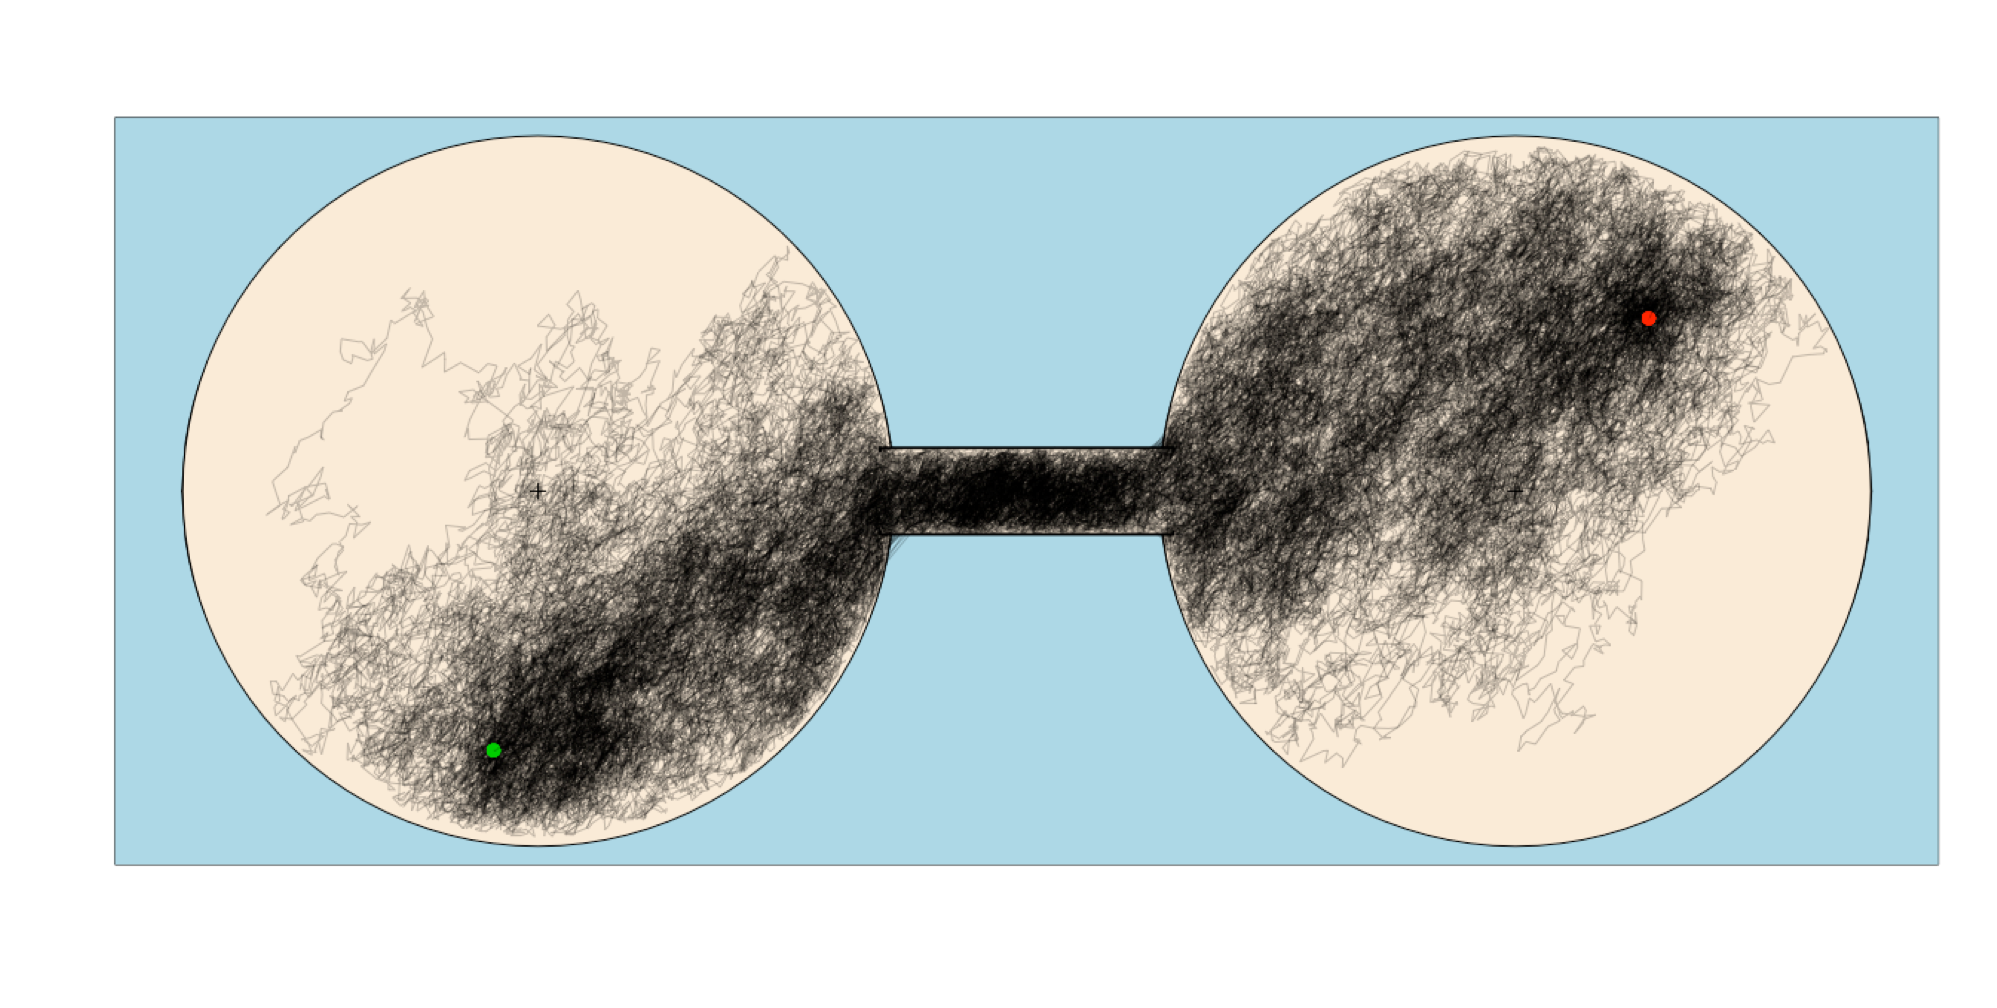
\includegraphics[width=160mm]{figures/biogeographic_diffusion.png}
\caption[Truncated Multivariate Brownian Motion in the Context of Biogeographic Diffusion]{An example of the truncated Brownian bridges between two tan islands surrounded by nigh-impassable ocean. Biogeographic diffusion began at the green dot and ended at the red dot, with multivariate Brownian paths of 0 correlation between the two sampled efficiently from their conditional distribution. \label{overflow} \label{fig:truncBrownMot}}
\end{figure*}
